\documentclass[12pt]{article}
\title{Maximal point problem}
\author{林橋毅 111502563}
\usepackage[UTF8]{ctex}
\usepackage{graphicx} %插入图片的宏包
\usepackage{float} %设置图片浮动位置的宏包
\usepackage{caption}
\usepackage{subfigure} %插入多图时用子图显示的宏包
\usepackage{algorithm}
\usepackage{cite}
\usepackage{algpseudocode}
\usepackage{amsmath}
\usepackage{graphics}
\usepackage{epsfig}
\usepackage{amssymb}
\usepackage{bm}
\newtheorem{definition}{Definition}

\begin{document}
\captionsetup[figure]{labelfont={bf}, labelformat={default}, labelsep=period,name={Fig.}}
\maketitle
\bibliographystyle{plain}
\part{Introduction}
最大點(Maximal point)問題是:找出點集合 S 中不被集合中任一一點支配的點,如果在點集合 S 中的兩個點 p 和 q,若 q 的每個維度的值皆大於等於 p 在該維度的值,我們則稱 q dominates p(q 支配 p)。\\

本篇基於二維最大點演算法的基礎上,使用分治的方法優化並實作出比暴力求解更有效率的三維最大點演算法,該演算法為$O(NlogN)$。

\begin{definition}
	Point \textbf{p} \textbf{dominates} point \textbf{q}, denoted by p $\prec$ q, if $x_i(p)$ >= $x_i(p)$ for i = 1,2,...d. (通常在 d <= 3 的情況下稱 $x_1$, $x_2$, $x_3$ 分別為 x, y, z)
\end{definition}

\begin{definition}
In a finite set of point S, point p $\in$ S is a \textbf{maximal point} if there does not exist a point q $\in$ S such that q \textbf{dominates} p.
\end{definition}


\part{Method}

\section{Two dimensionl}
求解二維最大點問題可以用以下掃描線的技巧求解(Fig. \ref{2DMaximal}),這個演算法可以分為以下步驟:
\begin{itemize}
	\item 將點以 x 座標由大到小排序
	\item 隨著 x 由大到小遍歷所有點並紀錄目前最大 y 座標,若遇到一點之 y 座標比目前紀錄最大值還大則此點是一個 Maximal point,將其輸出並更新最大的 y 座標。
\end{itemize}

\begin{figure}[H]
	\centering
	\includegraphics[width=0.6\textwidth]{2DMaximal}
	\caption{二維最大點問題示意圖 \cite{enwiki:1038770021}} %最终文档中希望显示的图片标题
	\label{2DMaximal} %用于文内引用的标签
\end{figure}

\begin{algorithm}[H]
	\caption{Pseudocode}
	\begin{algorithmic}
		\State sort point by x-corrdinate //將所有點依照 x 座標由大到小排序	好
		\State maxY = $p_0$ - 1
		\For{$i=0$ to $n$}
			\If{$p_i$ > maxY}
				\State M* $\leftarrow$ $p_i$
				\State maxY = $p_i$
			\EndIf
		\EndFor
	\end{algorithmic}
\end{algorithm}

\section{Three dimension}

\subsection{Brute force solution}
暴力求解法是直接對於點集合 S 的點用兩兩比較的方式,檢查每一個點是否被任何一點 dominates,如果沒有任何點可以支配他則此點為一個 Maximal point。(見附件 brute\_force.cpp)

\begin{algorithm}[H]
	\caption{Pseudocode}
	\begin{algorithmic}
		\State M* $\leftarrow$ $\varnothing$	// M* 用來儲存找到的 Maximal point
		\For{$i=0$ to $N$}
			\State flag = True
			\For{$j=0$ to $n$, i $\neq$ j}
				\If{point $p_j$ dominates point $p_i$}
					\State flag = False
				\EndIf
			\EndFor
			\If{flag == True}
				\State M* $\leftarrow$ $p_i$ // $p_i$ is a maximal point.
			\EndIf
		\EndFor
		\State sort(M*) //根據題目要求將 M* 排序好 
	\end{algorithmic}
\end{algorithm}

\subsection{Pruning solution}
觀察 3.1 的暴力求解法,我們可以觀察到,所有點無論如何都會被比較 N-1 次,但如果我們換個想法,紀錄點 $p$ 有沒有可能成為最大點,如果這個點 $p$ 不可能成為最大點時我們就可以直接跳過他,如果 $p$ 不可能成為最大點代表我們找到一個點 $q$ 可以 dominates $p$,並且所有 $p$ 可以支配的點 $q$ 也都可以支配,所以如果能夠確定 $p$ 不為最大點便可以將其標記起來,後續比較時可以直接跳過以加速比較過程,經過實驗相較於暴力求解確實在執行時間有提升。(見附件  pruning.cpp)

\begin{algorithm}[H]
	\caption{Pseudocode}
	\begin{algorithmic}
		\State M* $\leftarrow \varnothing$, check = {0}// M* 存最大點、check[i] 紀錄 $p_i$ 是否不可能為最大點
		\For{$i=0$ to $N$}
			\For{$j=0$ to $N$, i $\neq$ j and c[i] == 0}
					\If{$p_i$ dominates $p_j$}
				\State c[i] = 1
				\EndIf
			\EndFor
		\EndFor
		\State M* $\leftarrow p_i$ for check[i] == 0
		\State sort(M*)
	\end{algorithmic}
\end{algorithm}

\subsection{Divide and conquer algorithm}
基於二維的求解,可以將有序的三維點切分成許多個二維的平面,分別求解每個平面再將每個結果合併起來(Fig. \ref{3DMaximal})。用 $M_i$ 紀錄 $x=i$ 平面的最大點集,接著隨著座標由大到小維護一個做為答案的最大點集 M*,若 $\neg$ p $\prec$ M*,就將 p 放入 M*。(見附件 devide\_conquer.cpp)


\begin{definition}
	Finite set of point S, point p $\prec$ S if $\exists$ point q $\in S$ such that q dominates p.
\end{definition}


\begin{figure}[H]
	\centering
	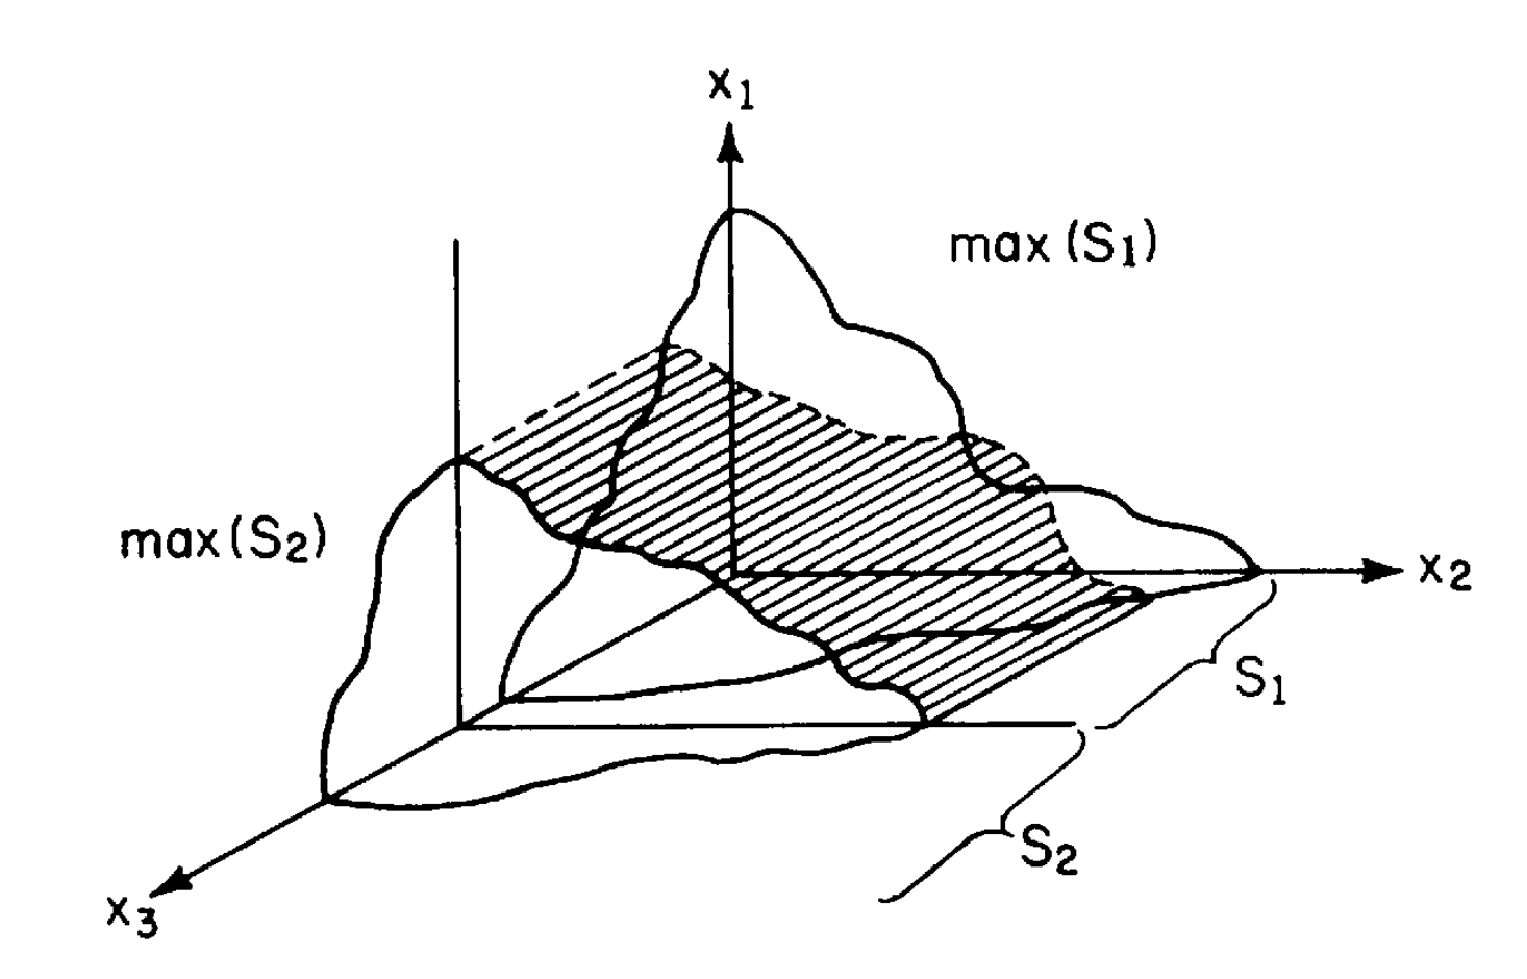
\includegraphics[width=0.6\textwidth]{3DMaximal}
	\caption{分治法示意圖\cite{Computational_geometry}。資料來源:Computational geometry p.162} %最终文档中希望显示的图片标题
	\label{3DMaximal} 
\end{figure}

\begin{algorithm}[H]
	\caption{Pseudocode}
	\begin{algorithmic}
		\State M $\leftarrow \varnothing$, M* $\leftarrow \varnothing$ // M 存每個平面的最大點、M* 為答案的最大點集合
		\State sort(p) // 將點排序好(x 由大到小若相等則 y 由大到小,依此類推...)
		\State Zmax = $p_0$ - 1 
		\For{$i=0$ to  $N$}
			\If{i $\neq$ 0 and $p_i.x$ != $p_{i-1}.x$}
				\State Zmax = $p_i.x -1$
			\EndIf
			\If{$p_i.z$ > Zmax}
				\State Zmax = $p_i.z$
				\State M $\leftarrow p_i$
			\EndIf
		\EndFor
		\For{$i=0$ to $M.size$}
			\If{$\neg (p_i \prec M*)$}
				\State $M* \leftarrow p_i$
			\EndIf
		\EndFor
	\end{algorithmic}
\end{algorithm}
\part{Experimental result}
我產生點座標範圍為 0 到 100000 的隨機測資(見附件 generator.cpp),測試從 N = 1 到 N = 20000 的時間表現,可以看到不管是剪枝法還是分治法都相對於暴力求解有優秀的效能提升。
\begin{figure}[H]
	\centering
	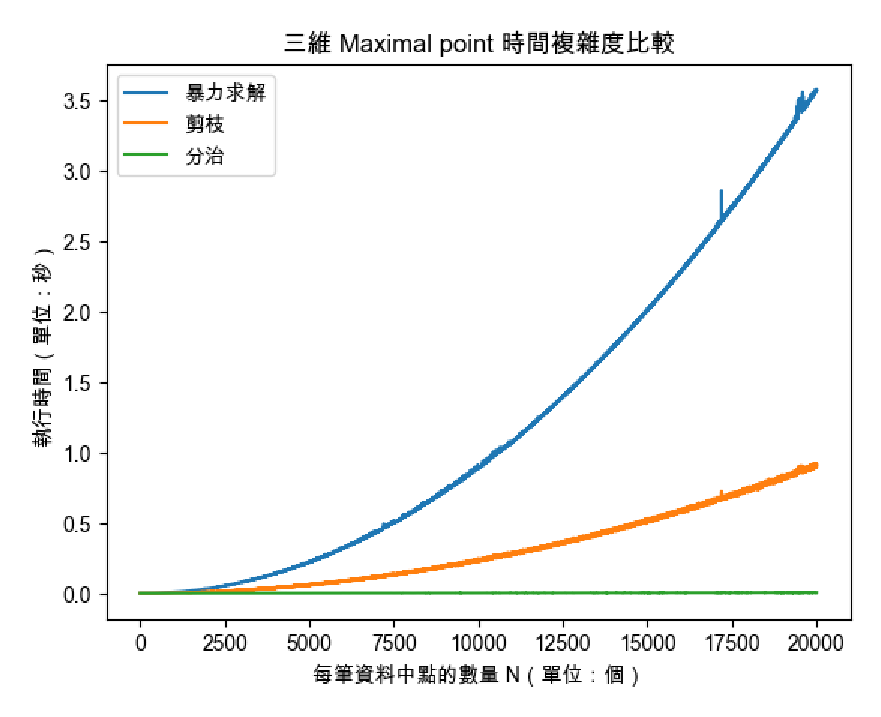
\includegraphics[width=0.7\textwidth]{time_compare}
	\caption{演算法時間複雜度比較圖} %最终文档中希望显示的图片标题
	\label{Fig.main1} %用于文内引用的标签
\end{figure}

\begin{figure}[H]
	\centering
	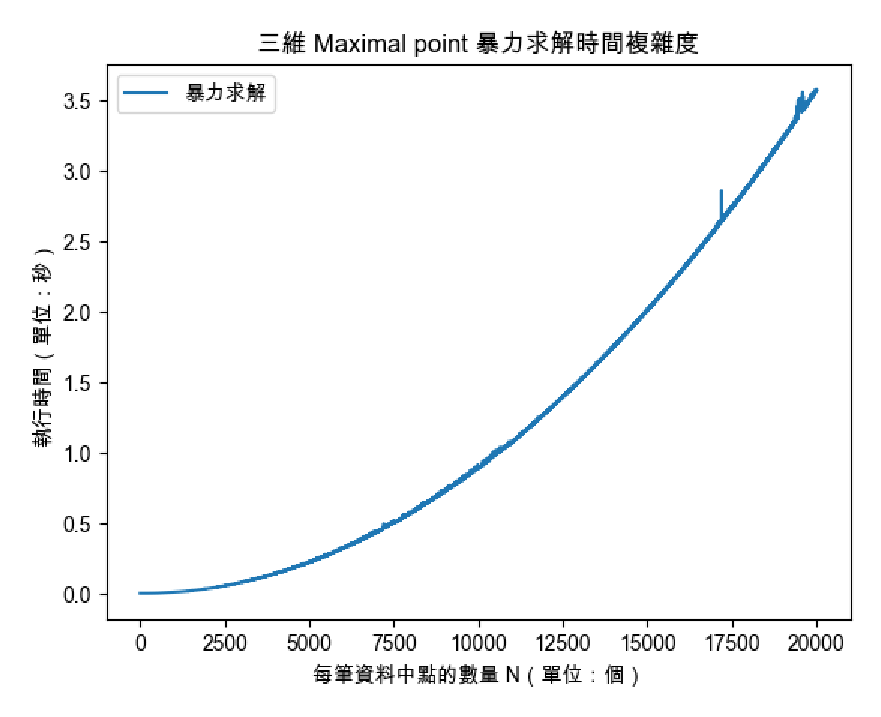
\includegraphics[width=0.7\textwidth]{bruteforce}
	\caption{暴力求解法執行時間圖} %最终文档中希望显示的图片标题
	\label{Fig.main2} %用于文内引用的标签
\end{figure}
\begin{figure}[H]
	\centering
	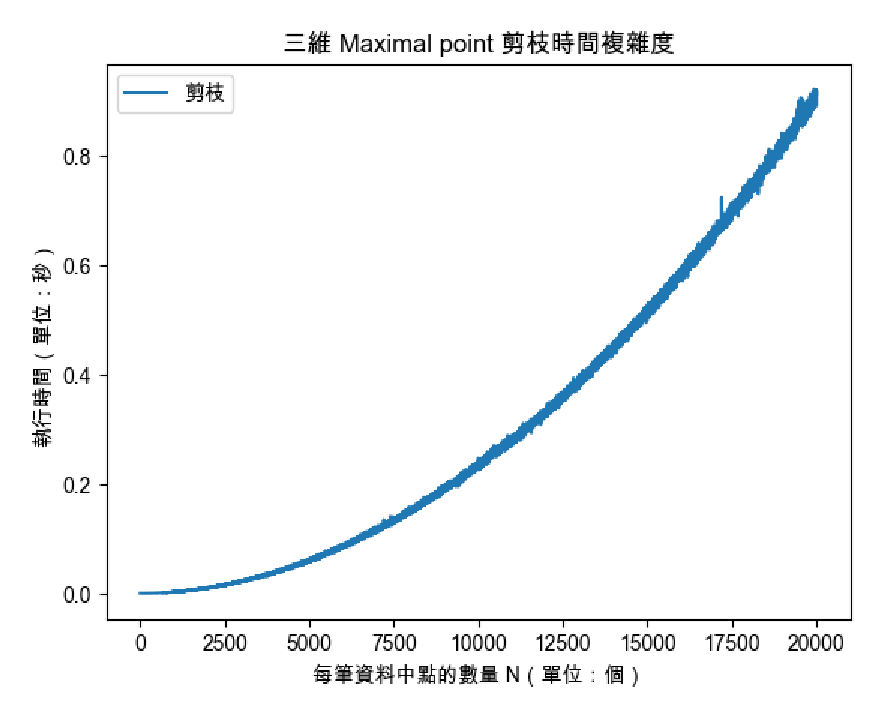
\includegraphics[width=0.7\textwidth]{pruning}
	\caption{剪枝法執行時間圖} %最终文档中希望显示的图片标题
	\label{Fig.main3} %用于文内引用的标签
\end{figure}
\begin{figure}[H]
	\centering
	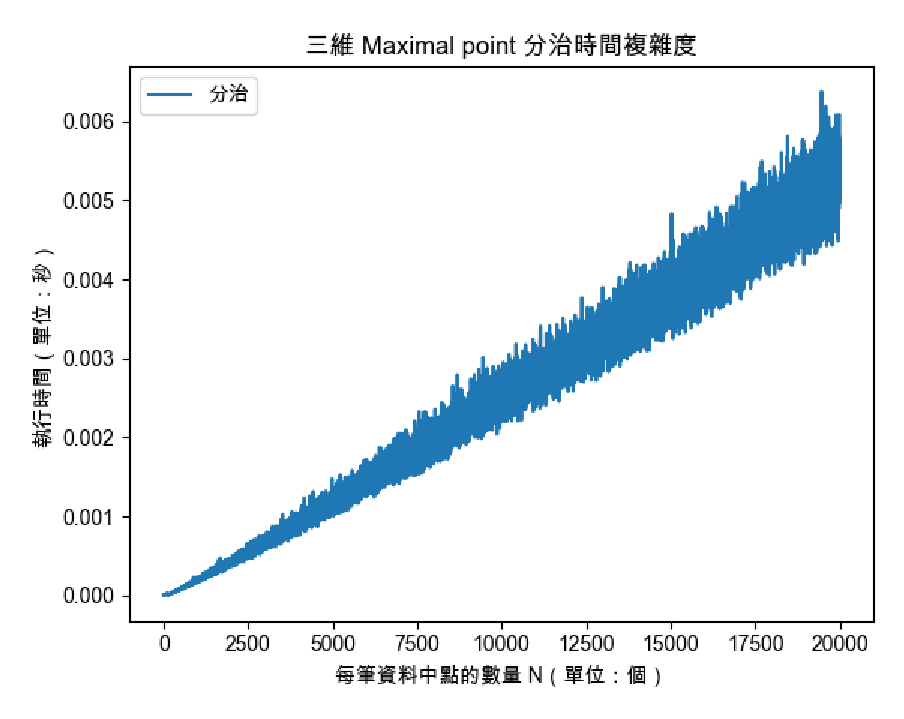
\includegraphics[width=0.7\textwidth]{linear}
	\caption{分治法執行時間圖} %最终文档中希望显示的图片标题
	\label{Fig.main4} %用于文内引用的标签
\end{figure}

\part{Conclusion}
本篇實作了兩種比暴力求解更快的演算法,分別是基於暴力求解的剪枝法優化暴力求解的速度,以及基於二維最大點問題使用分治法實現$O(NlogN)$的演算法。\\

分治法實現了$O(NlogN)$時間複雜度的演算法,相較暴力求解有優異的表現,在本篇所附上的程式碼若輸入之所有點都是 Maximal point 的狀況時,程式執行瓶頸將會落在維護最大點集合的部分,但在 N 較大時這個演算法的複雜度根據定義仍為 $O(NlogN)$\cite{Computational_geometry}\cite{enwiki:1038770021} ,且實驗當中也可以驗證此結果,未來能夠用 AVL Tree 維護以改善這個缺點。

未來期望能夠證明出空間中 Maximal point 的最大數量後可以得出更嚴謹的時間複雜度證明。最後,也展望未來能夠繼續研究並且實作高維度的 Maximal point 問題。

\bibliography{reference}

\end{document}